\documentclass[11pt, a4paper]{article}
\usepackage{amsmath, amssymb}
\usepackage{graphicx}
\usepackage{tikz}
\usetikzlibrary{shapes, arrows, arrows.meta, positioning, fit, calc, backgrounds}
\usepackage{geometry}
\geometry{margin=1in}
\usepackage{hyperref}
\usepackage{caption}
\usepackage{lmodern}

\begin{document}

\title{\textbf{MAPPO with GAT Actor and Transformer Critic \\ Architecture Details}}
\author{}
\date{}
\maketitle

\section{Overview}
The reinforcement learning setup employs a Multi-Agent Proximal Policy Optimization (MAPPO) framework. The architecture is split into a decentralized Graph Attention Network (GAT) Actor and a centralized Transformer Critic. The model is specifically designed for the GPSD-Conn environment, incorporating topological features like the Fiedler value for maintaining connectivity.

\section{Decentralized GAT Actor (\texttt{GATActor})}
The Actor network operates decentrally, utilizing only the local observation of each agent. It extracts self-features and neighborhood features, constructs a local communication graph based on the communication radius $r_c$, and applies Graph Attention layers to aggregate neighborhood information.

\subsection{Architecture Details}
\begin{figure}[h]
\centering
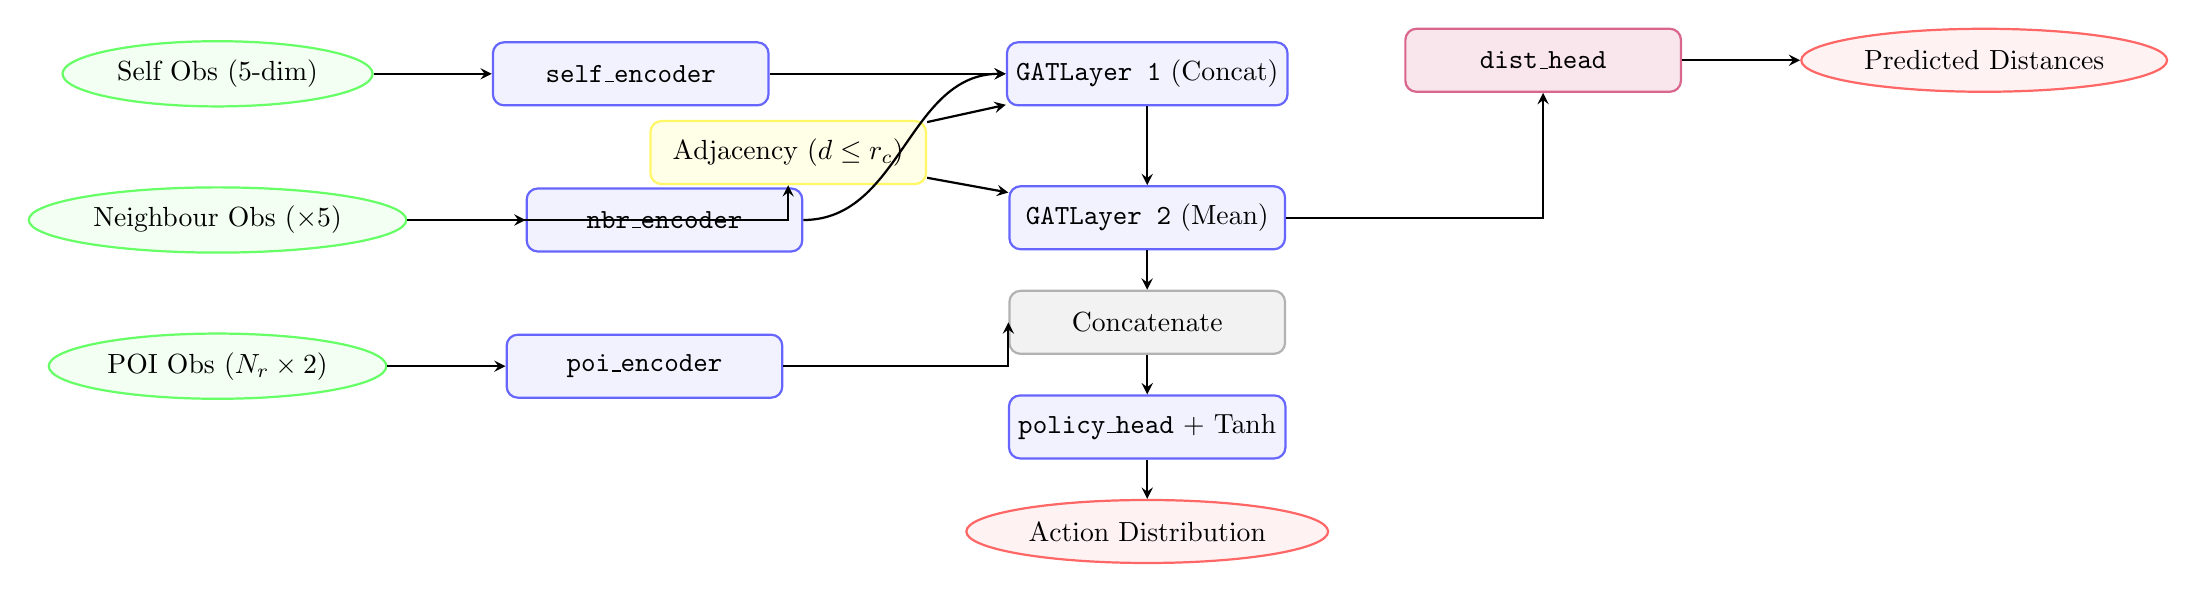
\begin{tikzpicture}[
    node distance=1cm and 1.5cm,
    layer/.style={rectangle, draw=blue!60, fill=blue!5, thick, minimum width=3.5cm, minimum height=0.8cm, align=center, rounded corners},
    input/.style={ellipse, draw=green!60, fill=green!5, thick, minimum width=3cm, minimum height=0.8cm, align=center},
    output/.style={ellipse, draw=red!60, fill=red!5, thick, minimum width=3cm, minimum height=0.8cm, align=center},
    arrow/.style={->, thick, >=stealth}
]

% Inputs
\node[input] (self_obs) {Self Obs (5-dim)};
\node[input, below=of self_obs] (nbr_obs) {Neighbour Obs ($\times 5$)};
\node[input, below=of nbr_obs] (poi_obs) {POI Obs ($N_r \times 2$)};

% Encoders
\node[layer, right=of self_obs] (self_enc) {\texttt{self\_encoder}};
\node[layer, right=of nbr_obs] (nbr_enc) {\texttt{nbr\_encoder}};
\node[layer, right=of poi_obs] (poi_enc) {\texttt{poi\_encoder}};

% GAT
\node[layer, right=of self_enc, xshift=1.5cm] (gat1) {\texttt{GATLayer 1} (Concat)};
\node[layer, below=of gat1] (gat2) {\texttt{GATLayer 2} (Mean)};

% Auxiliary
\node[layer, right=of gat2, yshift=2.0cm, fill=purple!10, draw=purple!60] (dist_head) {\texttt{dist\_head}};
\node[output, right=of dist_head] (dist_pred) {Predicted Distances};

% Graph formulation
\node[layer, fill=yellow!10, draw=yellow!60, left=of gat1, xshift=0.5cm, yshift=-1.0cm] (graph) {Adjacency ($d \leq r_c$)};

% Aggregation
\node[layer, fill=gray!10, draw=gray!60, below=of gat2, xshift=0cm, yshift=0.5cm] (concat) {Concatenate};

% Policy Head
\node[layer, below=of concat, yshift=0.5cm] (policy_head) {\texttt{policy\_head} + Tanh};
\node[output, below=of policy_head, yshift=0.5cm] (action) {Action Distribution};

% Connections
\draw[arrow] (self_obs) -- (self_enc);
\draw[arrow] (nbr_obs) -- (nbr_enc);
\draw[arrow] (poi_obs) -- (poi_enc);

\draw[arrow] (nbr_obs) -| (graph);
\draw[arrow] (self_enc) -- (gat1);
\draw[arrow] (graph) -- (gat1);
\draw[arrow] (graph) -- (gat2);

\draw[arrow] (nbr_enc.east) to[out=0, in=180] (gat1.west); 

\draw[arrow] (gat1) -- (gat2);
\draw[arrow] (gat2.east) -| (dist_head.south);
\draw[arrow] (dist_head.east) -- (dist_pred.west);

\draw[arrow] (gat2.south) -- (concat.north);
\draw[arrow] (poi_enc.east) -| (concat.west);

\draw[arrow] (concat.south) -- (policy_head.north);
\draw[arrow] (policy_head.south) -- (action.north);

\end{tikzpicture}
\caption{Decentralized Graph Attention Actor.}
\end{figure}

\section{Centralized Transformer Critic (\texttt{TransformerCritic})}
The Critic network evaluates the state using full observability during training. It employs a Transformer Encoder to perform self-attention across all agents' local observations and centralized topological metrics like the Fiedler value.

\subsection{Architecture Details}
\begin{figure}[h]
\centering
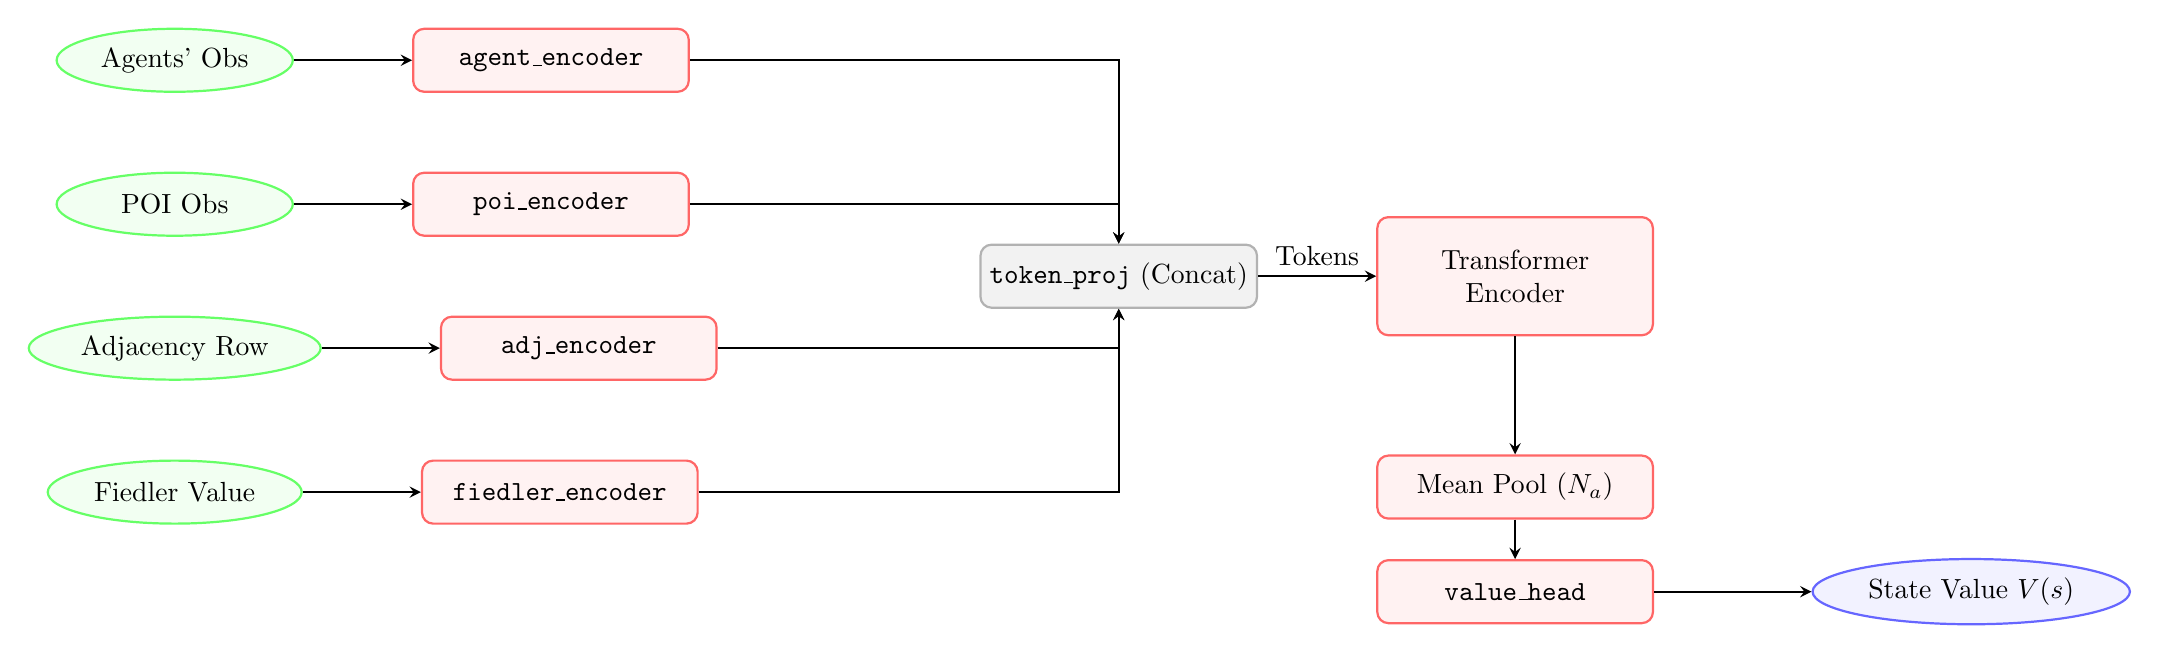
\begin{tikzpicture}[
    node distance=1cm and 1.5cm,
    layer/.style={rectangle, draw=red!60, fill=red!5, thick, minimum width=3.5cm, minimum height=0.8cm, align=center, rounded corners},
    input/.style={ellipse, draw=green!60, fill=green!5, thick, minimum width=3cm, minimum height=0.8cm, align=center},
    output/.style={ellipse, draw=blue!60, fill=blue!5, thick, minimum width=3cm, minimum height=0.8cm, align=center},
    arrow/.style={->, thick, >=stealth}
]

% Inputs
\node[input] (agent_obs) {Agents' Obs};
\node[input, below=of agent_obs] (poi_obs) {POI Obs};
\node[input, below=of poi_obs] (adj_obs) {Adjacency Row};
\node[input, below=of adj_obs] (fiedler_obs) {Fiedler Value};

% Encoders
\node[layer, right=of agent_obs] (agent_enc) {\texttt{agent\_encoder}};
\node[layer, right=of poi_obs] (poi_enc) {\texttt{poi\_encoder}};
\node[layer, right=of adj_obs] (adj_enc) {\texttt{adj\_encoder}};
\node[layer, right=of fiedler_obs] (fiedler_enc) {\texttt{fiedler\_encoder}};

% Aggregation
\coordinate (center) at ($(poi_enc.south east) !0.5! (adj_enc.north east)$);
\node[layer, fill=gray!10, draw=gray!60, right=of center, xshift=2cm] (token_proj) {\texttt{token\_proj} (Concat)};

% Transformer
\node[layer, right=of token_proj, yshift=0cm, minimum height=1.5cm] (transformer) {Transformer\\Encoder};

% Pooling & Value
\node[layer, below=of transformer, yshift=-0.5cm] (pool) {Mean Pool ($N_a$)};
\node[layer, below=of pool, yshift=0.5cm] (val_head) {\texttt{value\_head}};
\node[output, right=of val_head, xshift=0.5cm] (value) {State Value $V(s)$};

% Connections
\draw[arrow] (agent_obs) -- (agent_enc);
\draw[arrow] (poi_obs) -- (poi_enc);
\draw[arrow] (adj_obs) -- (adj_enc);
\draw[arrow] (fiedler_obs) -- (fiedler_enc);

\draw[arrow] (agent_enc.east) -| (token_proj.north);
\draw[arrow] (poi_enc.east) -| (token_proj.north);
\draw[arrow] (adj_enc.east) -| (token_proj.south);
\draw[arrow] (fiedler_enc.east) -| (token_proj.south);

\draw[arrow] (token_proj.east) -- (transformer.west) node[midway, above] {Tokens};
\draw[arrow] (transformer.south) -- (pool.north);
\draw[arrow] (pool.south) -- (val_head.north);
\draw[arrow] (val_head.east) -- (value.west);

\end{tikzpicture}
\caption{Centralized Transformer Critic.}
\end{figure}

\section{Additional Training Signals \& Details}
\begin{itemize}
    \item \textbf{Contrastive Auxiliary Task}: The actor uses an auxiliary head (\texttt{dist\_head}) to predict the distance to neighboring agents using the final GAT embedding. This enforces spatial awareness in the actor's latent representations. A coefficient (\texttt{contrastive-coef}) scales this loss.
    \item \textbf{Curriculum Learning for Connectivity}: The environment utilizes reward shaping where the penalty for disconnecting communication ramps up over the course of training (\texttt{conn-penalty-start} to \texttt{conn-penalty-end}).
    \item \textbf{Action Squashing}: The policy head outputs unbounded logits which are squashed through a \texttt{Tanh} activation and scaled by a learnable parameter (\texttt{logit\_scale}). This ensures the generated actions map smoothly to the defined action space bounds.
    \item \textbf{Value Normalization (PopArt-lite)}: The value target is normalized iteratively online to stabilize critic learning and accommodate dynamically shifting returns.
\end{itemize}

\end{document}
